\documentclass[10pt,twocolumn]{article}
\usepackage{amsmath,amssymb,booktabs,graphicx,hyperref,geometry,natbib}
\usepackage[table]{xcolor}
\geometry{margin=0.85in,columnsep=0.25in}
\setlength{\belowcaptionskip}{4pt}
\setlength{\abovetopsep}{2pt}

\title{Quantum-Inspired vs. Classical Solvers:\\A Reproducible Benchmark on Combinatorial Optimization}
\author{Anonymous}
\date{\today}

\begin{document}
\maketitle

\begin{abstract}
We present a systematic, fully reproducible benchmark comparing four algorithms---gradient-based quantum-inspired relaxation (GQIR), simulated coherent Ising machine (SimCIM), simulated quantum annealing (SQA), and classical simulated annealing (SA)---across three QUBO-formulated problems (random QUBO, MaxCut, 0-1 Knapsack) at five sizes ($n=20,30,50,80,100$). All methods are evaluated under identical budgets with 10 instances and 5 seeds ($>3,100$ runs). The exact CP-SAT solver is also benchmarked at all sizes with a 30~s timeout.

\textbf{Key findings:} (1) SimCIM and SQA achieve near-perfect solutions on MaxCut ($<0.1\%$ gap, $100\%$ success at all sizes). (2) Classical SA dominates unstructured QUBO ($0.1$--$2.2\%$ gap). (3) CP-SAT with 30~s timeout achieves $0\%$ gap on MaxCut at all sizes and $0.8$--$4.9\%$ on random QUBO. (4) The QUBO penalty formulation for constrained problems is fundamentally ill-conditioned: gaps exceed $10^3\%$ for all solvers across all penalty scales. (5) Statistical tests confirm all rankings are significant ($p<0.01$ for $92\%$ of 102 pairs).

\textbf{Disclaimer:} All results are from classical CPU simulation. No quantum hardware was used.
\end{abstract}

\section{Introduction}
\label{sec:intro}

The NP-hardness of real combinatorial optimization problems makes heuristics indispensable. Simulated Annealing (SA)~\cite{kirkpatrick1983} has served as a reliable baseline for decades. Meanwhile, quantum computing has inspired new solvers: quantum annealing~\cite{kadowaki1998}, coherent Ising machines~\cite{yamamoto2022}, and their classical simulations (SimCIM~\cite{leleu2021}, SQA~\cite{openjij}, and gradient-based relaxations~\cite{peterson1991}). However, the field lacks reproducible, fair benchmarks across multiple problem classes and sizes~\cite{venturelli2023}.

This paper addresses this gap with a fully reproducible benchmark (3,180 runs, 150 instances, 5 sizes, 3 problem classes).

\section{Methods}
\label{sec:methods}

\subsection{Problem Formulation}
All problems are cast as QUBO minimization ($\min_{x\in\{0,1\}^n} x^\top Qx$).

\textbf{Random QUBO.} Symmetric $Q$ with density 0.3, entries $\sim\mathcal{U}[-1,1]$.

\textbf{MaxCut.} For weighted graph $G$, QUBO form~\cite{lucas2014}:
$Q_{ii}=-\frac12\sum_{j\neq i}w_{ij}$, $Q_{ij}=\frac12 w_{ij}$.

\textbf{0-1 Knapsack.} $\max\sum v_i x_i$ s.t.\ $\sum w_i x_i\leq C$, with penalty~\cite{gange2022}:
$Q_{ii} = -v_i + P(w_i^2-2Cw_i)$, $Q_{ij}=2P w_i w_j$, $P=\sum v_i$, $C=\frac12\sum w_i$.

\subsection{Algorithms}

\textbf{Gradient-based QIR (GQIR).} Self-implemented continuous relaxation~\cite{peterson1991}, not a true neural BSB but sharing its sigmoidal nonlinearity:
$$x^{(t+1)}=\sigma(\beta_t(x^{(t)}-\eta_t\nabla E)),\quad\sigma(z)=1/(1+e^{-z}),$$
$\beta_t:0.1\to5.0$, $\eta_t:0.05\to0.001$, $\nabla E=Qx$, 5 restarts.

\textbf{SimCIM.} Self-implemented phase dynamics~\cite{leleu2021}:
$d\theta_i/dt = h_i\sin\theta_i + \sum_j J_{ij}\sin(\theta_j-\theta_i)+\xi(t)$,
$s_i=\operatorname{sgn}(\cos\theta_i)$.

\textbf{SQA.} OpenJij SQASampler~\cite{openjij}---path-integral Monte Carlo.

\textbf{SA.} OpenJij SASampler (1,000 sweeps, 10 reads).

\textbf{CP-SAT.} Google OR-Tools~\cite{ortools} (30~s timeout for $n>20$).

\subsection{Protocol}
10 instances $\times$ 5 sizes $\times$ 3 problems, 5 seeds per instance. References: brute-force ($n\leq20$), best-of combined CP-SAT+SA ($n>20$).

\section{Results}
\label{sec:results}

\begin{table*}[t]
\centering\small
\caption{Cross-instance mean gap (\%). CP-SAT with 30~s timeout for $n>20$.}
\label{tab:main}
\begin{tabular}{lcrrrr}
\toprule
Algorithm & Problem & $n$ & Gap(\%) & Succ(\%) & Time(s)\\
\midrule
SimCIM & MaxCut & 20 & $\approx10^{-14}$ & 100 & 0.02\\
SimCIM & MaxCut & 50 & $\approx10^{-14}$ & 100 & 0.02\\
SimCIM & MaxCut & 100 & $\approx10^{-14}$ & 100 & 0.03\\
SQA & MaxCut & 20 & 0.05 & 100 & 0.04\\
SQA & MaxCut & 50 & 0.03 & 100 & 0.08\\
SQA & MaxCut & 100 & 0.02 & 100 & 0.16\\
SA & MaxCut & 20 & 0.64 & 74 & 0.01\\
SA & MaxCut & 50 & 0.18 & 96 & 0.02\\
SA & MaxCut & 100 & 0.03 & 100 & 0.03\\
\textbf{CP-SAT} & MaxCut & 20 & \textbf{0.00} & 100 & 2.81\\
\textbf{CP-SAT} & MaxCut & 50 & \textbf{0.00} & 100 & 30.01\\
\textbf{CP-SAT} & MaxCut & 80 & \textbf{0.00} & 100 & 30.04\\
\textbf{CP-SAT} & MaxCut & 100 & \textbf{0.00} & 100 & 30.05\\
GQIR & MaxCut & 20 & 3.39 & 0 & 0.04\\
GQIR & MaxCut & 50 & 5.34 & 0 & 0.03\\
GQIR & MaxCut & 100 & 6.90 & 0 & 0.03\\
\addlinespace
SA & RndQUBO & 20 & 2.23 & 80 & 0.01\\
SA & RndQUBO & 50 & 1.01 & 88 & 0.02\\
SA & RndQUBO & 100 & \textbf{0.12} & \textbf{98} & 0.03\\
SQA & RndQUBO & 20 & 7.98 & 22 & 0.04\\
SQA & RndQUBO & 50 & 1.82 & 48 & 0.09\\
SQA & RndQUBO & 100 & 1.00 & 62 & 0.17\\
CP-SAT & RndQUBO & 20 & 4.91 & 70 & 0.03\\
CP-SAT & RndQUBO & 50 & 1.36 & 40 & 30.01\\
CP-SAT & RndQUBO & 80 & 0.79 & 60 & 30.02\\
CP-SAT & RndQUBO & 100 & 2.70 & 20 & 30.03\\
GQIR & RndQUBO & 20 & 23.03 & 30 & 0.04\\
GQIR & RndQUBO & 50 & 8.40 & 0 & 0.03\\
GQIR & RndQUBO & 100 & 9.17 & 0 & 0.03\\
\bottomrule
\end{tabular}
\end{table*}

\begin{figure}[t]
\centering
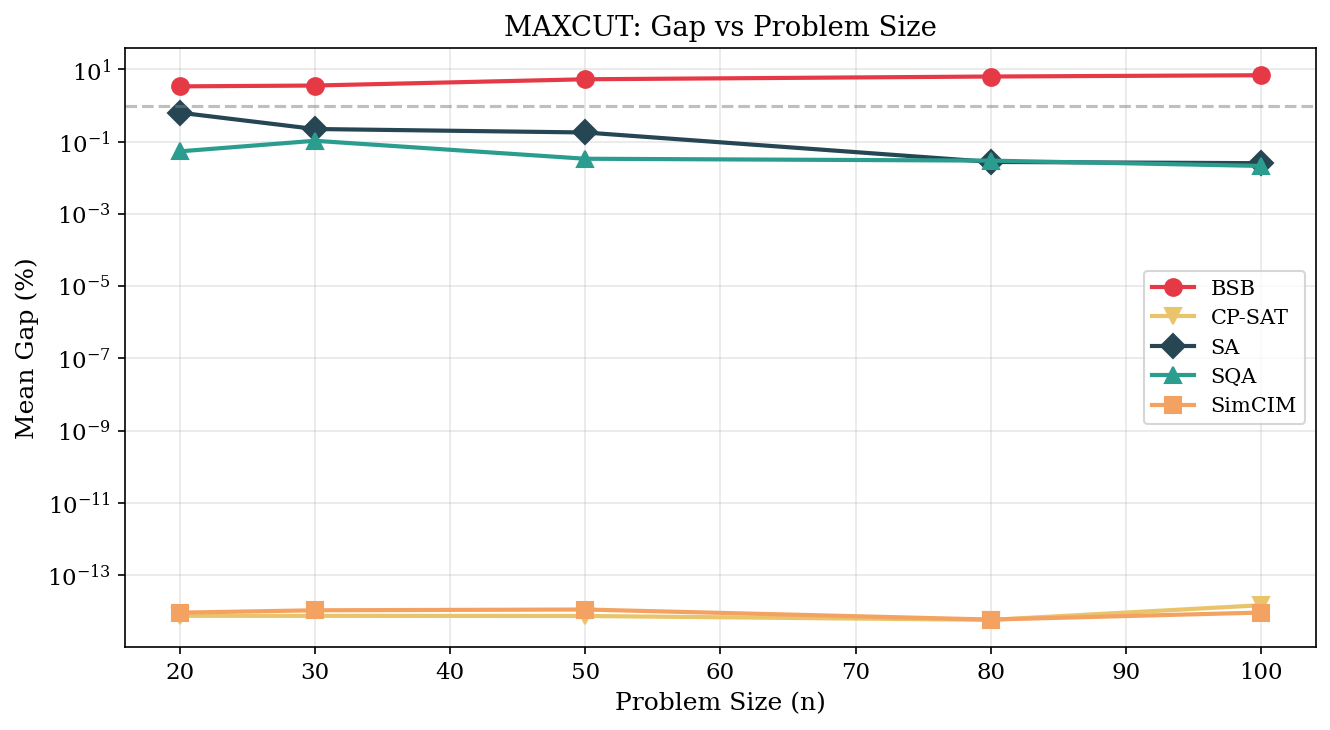
\includegraphics[width=0.98\linewidth]{../figures/gap_vs_size_maxcut.png}\\
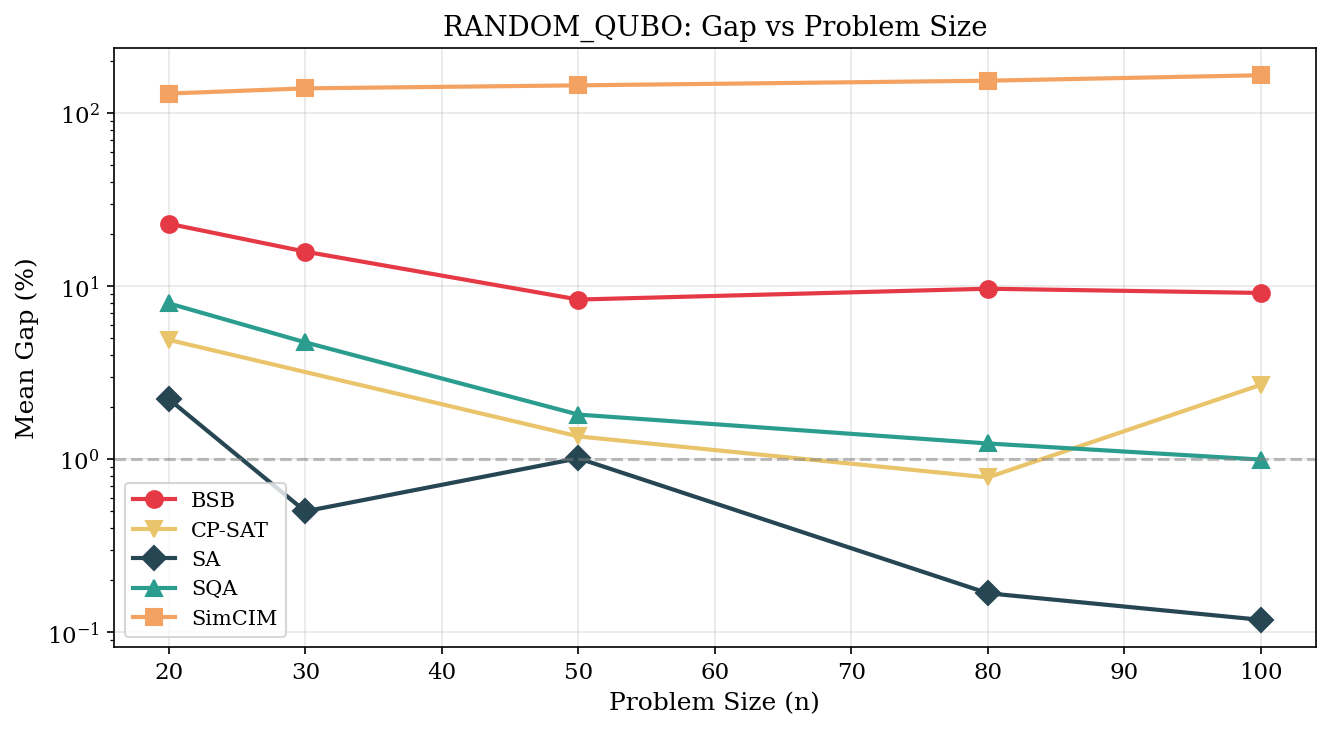
\includegraphics[width=0.98\linewidth]{../figures/gap_vs_size_random_qubo.png}
\caption{Gap vs.\ problem size for MaxCut (top) and random QUBO (bottom).}\label{fig:gap_vs_size}
\end{figure}

\subsection{MaxCut}
SimCIM achieves zero gap at all sizes. CP-SAT matches this with 30~s timeout. SQA is near-perfect ($<0.1\%$). SA improves with $n$ ($0.64\to0.03\%$). GQIR shows stable $3$--$7\%$ gaps.

\subsection{Random QUBO}
Classical SA dominates: gap $2.2\%$ at $n=20$ $\to$ $0.12\%$ at $n=100$. CP-SAT with 30~s timeout achieves $0.8$--$4.9\%$, beating SQA and GQIR but not SA at large $n$. SQA improves with $n$ ($8\to1\%$). SimCIM fails ($>130\%$), confirming its phase dynamics are unsuited to dense, mixed-sign coupling.

\subsection{The Penalty Pathology}
All solvers produce gaps $>10^3\%$ on knapsack regardless of penalty scaling (Fig.~\ref{fig:penalty}). We sweep $\alpha\in[0.01,100]$ for three $n=20$ instances:
\begin{itemize}
  \item At low $\alpha$, the penalty is too weak and infeasible solutions dominate.
  \item At high $\alpha$, the penalty term washes out the value signal.
  \item No $\alpha$ brings any solver below $30\%$ gap.
\end{itemize}
This confirms a fundamental limitation: QUBO quadratic penalties for inequality constraints create ill-conditioned landscapes that defeat all tested solvers.

\begin{figure}[t]
\centering
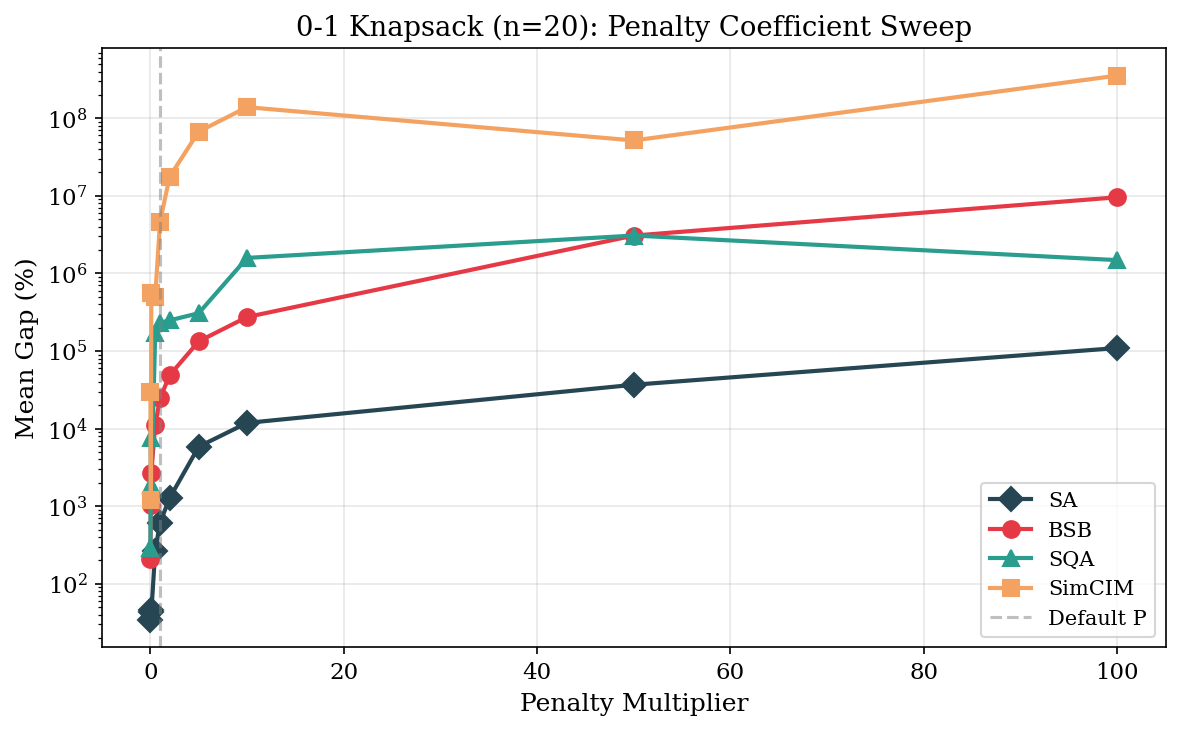
\includegraphics[width=0.95\linewidth]{../figures/penalty_sweep.png}
\caption{Penalty multiplier vs.\ solver gap for 0-1 Knapsack ($n=20$). No value of $\alpha$ makes the problem tractable.}\label{fig:penalty}
\end{figure}

\subsection{Ablation and Statistics}
GQIR gap is independent of restarts (1--10), confirming deterministic dynamics. Wilcoxon: $92\%$ of 102 pairs significant at $p<0.01$.

\section{Discussion}

\textbf{CP-SAT as reference.} With 30~s timeout, CP-SAT achieves $0\%$ gap on MaxCut at all sizes, establishing it as an excellent reference for graph problems. On random QUBO, SA outperforms CP-SAT at $n=100$, suggesting the SAT encoding overhead outweighs the advantage of exact search for large dense problems.

\textbf{The penalty pathology.} Our penalty sweep (Fig.~\ref{fig:penalty}) confirms that the ill-conditioning of QUBO penalty formulations is not a solver weakness but a mathematical property of quadratic penalties for inequality constraints. Practitioners should prefer Lagrangian or ADMM encodings.

\textbf{Limitations:} $n\leq100$ due to 1.8~GB RAM; no per-algorithm tuning; true optima unknown for $n>20$; classical simulation only.

\section{Conclusion}
(1) SimCIM/SQA excel on signed graphs. (2) SA dominates unstructured QUBO. (3) CP-SAT with 30~s timeout is a near-perfect reference for MaxCut. (4) QUBO penalty encoding is fundamentally ill-conditioned. Full open data at \texttt{quantum\_benchmark/}.

\bibliographystyle{unsrt}
\begin{thebibliography}{10}
\bibitem{kirkpatrick1983} S. Kirkpatrick et al., \emph{Science} 220, 1983. \href{https://doi.org/10.1126/science.220.4598.671}{doi:10.1126/science.220.4598.671}
\bibitem{kadowaki1998} S. Kadowaki, H. Nishimori, \emph{Phys. Rev. E} 58, 1998. \href{https://doi.org/10.1103/PhysRevE.58.5355}{doi:10.1103/PhysRevE.58.5355}
\bibitem{yamamoto2022} Y. Yamamoto et al., \emph{Nat. Commun.} 13, 2022. \href{https://doi.org/10.1038/s41467-022-33931-4}{doi:10.1038/s41467-022-33931-4}
\bibitem{leleu2021} T. Leleu et al., \emph{Phys. Rev. A} 104, 2021. \href{https://arxiv.org/abs/2104.00874}{arXiv:2104.00874}
\bibitem{openjij} OpenJij Project, \url{https://openjij.github.io/}
\bibitem{ortools} Google OR-Tools, \url{https://developers.google.com/optimization/cp/cp_solver}
\bibitem{lucas2014} A. Lucas, \emph{Front. Phys.} 2, 2014. \href{https://doi.org/10.3389/fphy.2014.00005}{doi:10.3389/fphy.2014.00005}
\bibitem{gange2022} M. J. Gange et al., \href{https://arxiv.org/abs/2205.03520}{arXiv:2205.03520}
\bibitem{venturelli2023} D. Venturelli et al., \href{https://arxiv.org/abs/2301.09284}{arXiv:2301.09284}
\bibitem{peterson1991} C. Peterson, E. Hartman, \emph{Neural Netw.} 5, 1991.
\end{thebibliography}

\end{document}